\section{Itthipaṇḍaka, Animittā, Nimittamattā, Vepurisikā}

There are various other words mentioned in the ordination procedures for {\em Bhikkhunīs} as described in the {\em Bhikkhunikkhandhaka} that are interesting in this context. The last three of these do not exclude an aspirant from ordination:\footnote{Khandhaka 20 Bhikkhunikkhandhaka PTS vol 2 page 271, translated by Ajahn Brahmali.} \\

\begin{tabular}{ l l }
 {\em itthipaṇḍaka} & female {\em paṇḍaka} \\
 {\em animittā } & woman who lacks genitals \\
 {\em nimittamattā } & woman with incomplete genitals \\ 
 {\em vepurisikā } & woman who is manlike \\
\end{tabular} \\

The word {\em animittā} literally means `signless' and appears a number of times in the Canon but mostly with a different meaning, namely as in {\em animitto (ceto)samādhi}, which is translated by Bhikkhu Sujato as `signless immersion', a term used in the context of meditation. In the context of not having genitals, it only appears in the Canon in the {\em Bhikkhunikkhandhaka} and as a form of abuse for women in the {\em Bhikkhu Saṃ­ghā­di­sesa­ 3}; never on its own but always in the same sequence of words of which the above are a few.

The words {\em nimittamattā} and {\em vepurisikā} are explained in the {\em Samantapāsādikā}\footnote{Sp.1.285, translations by Ajahn Brahmali}:
\begin{quote}
{\em Nimittamattāsīti tava itthinimittaṃ aparipuṇṇaṃ saññāmattamevāti vuttaṃ hoti.\\
...\\
Vepurisikāti samassudāṭhikā purisarūpā itthī.}
\end{quote}

\begin{quote}
You are a {\em nimittamattā}: you have incomplete female characteristics, merely a token.\\
...\\
{\em Vepurisikā} means a woman who has a beard and a mustache like a man.
\end{quote}

The first three of these terms terms in the {\em Bhikkhunikkhandhaka} are rather vague in their descriptions. The Chinese texts are not very clear on this point either but the overall questions asked here seem to have mostly to do with menstruation and diseases. At first glance it seems that the rules regarding ordination are trying to make sure that the girl in question is old enough for ordination and not ill. Rules concerning whether or not a girl has breasts can be explained as a question with regards to age, or it can be explained as a question to find out if she has developed the secondary characteristics needed or is possibly intersex. We will never know the true purpose behind these questions but it is not unlikely that these questions about the development of sexual organs were asked for the sole purpose of establishing age. After all, we also find rules in the {\em Bhikkhunīpātimokkha} that prohibit the ordination of married girls under the age of 12.\footnote{{\em Pācittiya 65 Yā pana bhikkhunī ūnad­vāda­sa­vassaṃ gihigataṃ vuṭṭhāpeyya, pācittiyaṃ.} (``Should any bhikkhuni give Acceptance to a married woman less than twelve years old, it is to be confessed.'', translation by Thanissaro Bhikkhu)} 

The question about whether a girl is sterile would point to her at least having had one child (how else would they know if she is able to conceive?) but this would seem strange if she wants to enter a celibate Order. It seems likely that the question was intended to establish if she is at least old enough to menstruate. Another possible explanation could be that women who could not conceive would be unable to marry or would be subject to divorce if the marriage remained barren. These women might have been considered outcastes and in order to survive and for protection might have sought refuge in the {\em Saṅgha}. The {\em Saṅgha} might have therefore set up these rules in order to prevent them getting inundated with candidates seeking ordination for the wrong reasons.\footnote{With sincere gratitude to Ajahn Brahmali for this suggestion.} There are several stories about nuns who sought refuge in the Buddhist or Jain {\em Saṅghas} after having been rejected by their husbands or were widowed. We find some of these stories in the {\em Therīgāthā}, the verses of the Senior Nuns, for instance in the story of {\em Isidāsī}\footnote{Thig 15.1.}, {\em Candā}\footnote{Thig 5.12.}, {\em Paṭācārā}\footnote{See \cite{hecker}.} or in the Jain scriptures in the story of Bhadda Kundalakesa.\footnote{See \cite{hecker}.}

The following table gives an overview of the terms:

\bigskip
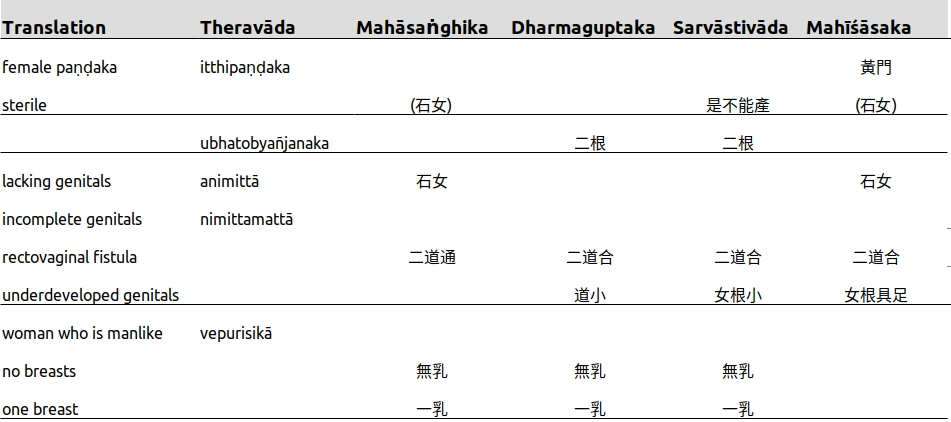
\includegraphics[width=\linewidth]{female.jpg}
\label{female}

These terms hardly appear in any texts or commentaries. Bhikkhu \cite{sujato2009} argues that the {\em Bhikkhunikkhandhaka}, as well as other parts of the Vinaya, are a later addition, possibly dating back to the Second Council and the elusiveness of these terms seems to confirm that. 

Note that in the Pali, the word used for characteristic in the ordination procedure is {\em nimitta} and not {\em liṅga} or {\em vyañ­jana} as we would expect. Bhikkhu Sujato points out that the Bhikkhunī Vinaya uses its own language and terminology that is often more in line with the Jain terminology and is poorly integrated with the Bhikkhu Vinaya.\footnote{\cite{sujato2009} page 143–145.} This could explain the discrepancies we see between the Bhikkhu and Bhikkhunī Vinaya in describing certain words pertaining to gender as used in the ordination procedures. In any case, the variability and vagueness of these terms with reference to gender do not permit a clear picture. 

It is certain though that the terms {\em paṇḍaka} and {\em ubhatob­yañ­janaka} pertained exclusively to male candidates as we have also seen in the Jain Order while the Bhikkhunī seem to have had their own vocabulary.

There are some rare cases of people who were raised from birth as girls that later became assigned as {\em hijra} after they failed to develop secondary female sexual characteristics (breast development and menstruation) at puberty.\footnote{See \cite{nanda} page 15.} Although there is very little evidence to go on, I believe that these cases could possibly be representing the {\em itthipaṇḍaka}. The term {\em itthipaṇḍaka} only appears in the Pali scriptures and in an early commentary of the Mūlasarvāstivāda Vinaya (黃門女). In the latter it seems to define it as either having no menstruation or not fully formed urinal tract\footnote{T24 1451 根本說一切有部毘奈耶雜事 0364b16 and 0364b27. With much gratitude to Dr. Hsiao-Lan Hu for pointing this out.}. The Mahīśāsaka Vinaya talks about a 黃門 ({\em paṇḍaka}) without adding the character for `female' (女). We also see a similar idea emerging in Tantric Hinduisim\footnote{See \cite{nanda} pages 21–22.} where a woman without menstruation is seen as a `female eunuch'.

At least in the Bhikkhunī ordination in the Theravāda lineage, the characteristics of an {\em animittā, nimittamattā or vepurisikā} do not invalidate an ordination. This is possibly also true in several of the Chinese Vinayas.
